% !Mode:: "TeX:UTF-8"

\chapter{基于换脸先验迁移的多目标自适应模型反演方法}[Model Inversion Attack Based on Face Swapping Prior Migration]\label{chap:MIA}

\section{引言}

模型反演攻击旨在从训练完成的分类模型中重建其训练数据的敏感特征。传统基于梯度优化的方法直接在像素空间进行优化,面临生成质量低下、优化效率不足等问题。近年来引入生成式先验可提升攻击效果,但现有工作在身份控制精度与生成保真度的平衡上仍存在不足。

本章将扩散换脸模型应用于模型反演攻击任务。换脸模型具有显式的身份属性解耦机制,但其标准推理流程依赖真实目标图像,而攻击场景中仅拥有类别标签。本章设计标签条件嵌入层、低秩适应微调、渐进式训练策略、多目标优化框架与分类器引导推理机制,将离散标签映射为连续身份嵌入,实现从类别标签到高保真攻击样本的生成。

本章首先形式化定义问题与威胁模型,随后阐述换脸先验模型的选择与适配改造、标签条件嵌入层设计、低秩适应微调策略、多目标优化损失函数框架与渐进式三阶段训练策略,最后给出完整的训练算法与分类器引导推理流程。基于上述方法,本章在VGGFace2、CelebA等标准数据集上进行系统实验,针对ArcFace、IR152与Face.evoLVe等不同架构的目标分类器评估攻击性能,通过与现有代表性方法的对比实验验证本章方法在攻击成功率与生成保真度上的优势,并通过消融实验量化各关键设计模块的性能贡献。

\section{形式化问题定义}
\label{sec:mia_problem}

根据第\ref{sec:thesis_structure}节建立的攻击任务框架,简要回顾模型反演攻击的形式化定义。设目标分类器为 $F_\theta:\mathcal{X}\to\mathbb{R}^C$,其中 $\mathcal{X}$ 为输入空间(如 $\mathbb{R}^{H\times W\times 3}$ 表示RGB图像),$C$ 为类别数量,$\theta$ 为模型参数。给定目标类别标签 $y_{\text{target}}\in\{1,2,\ldots,C\}$,攻击者的目标是生成图像集合 $\{\hat{x}_1, \hat{x}_2, \ldots, \hat{x}_K\}$,使其同时满足分类器认同度、感知真实性、身份相关性与多样性四个条件。完整的形式化定义与约束优化问题详见第\ref{sec:thesis_structure}节。

本章主要关注白盒威胁模型,即攻击者拥有目标分类器 $F_\theta$ 的完整信息,包括模型架构、参数以及完整的梯度信息 $\nabla_x F_\theta(x)$。这一威胁模型为评估模型的最大隐私泄露风险提供了上界,对应于模型开源、内部泄露或逆向工程成功的场景。在白盒设定下,攻击者可以直接利用梯度信息进行端到端优化:将分类器损失 $\mathcal{L}_{\text{cls}}(F_\theta(\hat{x}), y_{\text{target}})$ 融入生成模型的训练目标,通过反向传播更新生成器参数,使生成轨迹持续逼近目标类别的高置信区域。相比黑盒或灰盒场景(仅能查询输出概率),白盒访问权限提供了更强的优化信号,从而能够实现更高质量的重建结果。这一设定为深入研究方法设计与性能边界提供了理想的实验环境。

\section{基于换脸先验的反演架构与多目标优化损失}[Face-Swapping-Prior-Based Inversion Architecture and Multi-Objective Loss]
\label{sec:mia_architecture}

\subsubsection{换脸先验的选择与适配改造}

换脸模型作为本章方法的核心生成先验,需同时满足高质量身份迁移、显式身份-属性解耦与端到端可微分三项基本要求。相比传统的类条件生成先验,换脸模型在模型反演攻击任务中具有三方面本质优势。

传统类条件生成方法将类别标签直接作为条件输入生成模型,身份与属性隐式耦合在同一条件空间中,存在如下限制:(1)身份信息与姿态、表情、光照等属性维度缺乏明确分离,难以在保持目标身份一致性的同时生成多样化属性变化;(2)类条件生成先验通常需要在目标数据集上从零训练,缺乏大规模人脸先验知识,生成图像的细节保真度、面部结构合理性与身份特征一致性均受限;(3)类条件生成需要同时学习身份表示与属性生成两个复杂任务,优化难度高且容易出现模式崩溃。

相比之下,换脸模型通过参考注意力机制实现了身份与属性的显式解耦。具体而言,换脸模型将身份信息单独编码为嵌入向量,并通过专门设计的交叉注意力层注入生成过程,而姿态、表情、光照等属性信息则由源图像自然提供,两者在特征空间中保持独立。这种解耦机制带来三重优势:(1)身份特征可以在保持一致性的同时,通过不同源图像生成具有丰富属性变化的多样化样本,满足模型反演攻击任务对身份一致性与样本多样性的双重需求;(2)换脸模型在大规模人脸数据集上预训练,已经学习到丰富的面部结构先验、皮肤纹理、光影效果等细节知识,相比从零训练的类条件生成模型能够产生显著更高保真度的人脸图像;(3)通过利用源图像提供的属性信息,换脸模型将身份控制问题从"联合生成身份与属性"简化为"仅控制身份迁移",降低了优化复杂度并提高了训练稳定性。

鉴于换脸模型的上述优势,本章基于扩散模型的换脸方法REFace~\cite{sanoojan2024reface}构建生成先验。然而,其标准流程面向图像到图像的换脸任务,与模型反演攻击的输入形式存在根本性不兼容,需要系统性的架构改造与训练策略设计方能适配模型反演攻击场景。以下阐述换脸先验的适配挑战与本章提出的改造方案。

REFace的标准推理流程依赖真实的目标图像$x_{\text{target}}$作为身份参考,利用参考注意力机制将身份信息注入扩散去噪网络的每个时间步以实现身份控制。然而在模型反演攻击场景中,攻击者仅拥有目标类别的离散标签$y_{\text{target}}\in\{1,\ldots,C\}$,而无法获取任何真实的目标图像样本。这种输入模态的根本性差异构成了换脸先验应用于模型反演攻击的核心技术障碍,具体体现在三个方面:(1)标准换脸流程的身份嵌入来自图像编码器的实时提取,而模型反演攻击场景无图像输入,需从离散标签生成连续嵌入;(2)即使设计标签到嵌入的映射函数,其输出分布与ArcFace编码器在真实人脸图像上学习的嵌入分布存在显著差异,直接替换将导致换脸模型失效;(3)标准换脸任务优化感知相似度与身份保持度,而模型反演攻击需同时优化分类器置信度,两种目标在生成空间中可能相互竞争。上述挑战表明,换脸先验无法直接应用于模型反演攻击,必须进行深度改造。

针对前述挑战,本章提出三层次的系统性改造方案,将面向图像条件的换脸模型转化为支持标签条件的模型反演攻击工具:

(1)标签条件嵌入层设计:采用多层感知机架构将类别标签映射为连续身份嵌入向量,替代原有的ArcFace图像编码器,建立从离散标签空间到连续身份嵌入的可学习桥梁;

(2)低秩适应微调策略:针对标签嵌入的输出分布与真实图像ArcFace嵌入分布的显著差异,本章采用低秩适配技术,在冻结预训练主干的前提下,为关键层引入低秩可训练增量,以极小参数开销适配新的嵌入分布;

(3)渐进式训练与多目标优化:通过图像条件预热、混合条件过渡与纯标签条件适配三个阶段实现平滑的模态转换,同时采用任务不确定性加权框架统一管理多类优化目标。

该改造方案将面向图像条件、优化感知相似度的换脸模型,系统性地转化为面向标签条件、优化分类器置信度的模型反演攻击工具。以下各小节依次详细阐述这三层改造模块的技术细节与实现方法。

\subsection{整体架构设计}

\begin{figure}[!htbp]
  \centering
  \begin{tikzpicture}[scale=0.75, transform shape, node distance=1.3cm, >=stealth, thick,
    module/.style={rectangle, draw=blue!60, fill=blue!10, minimum width=2.5cm, minimum height=0.75cm, align=center, rounded corners},
    input/.style={rectangle, draw=green!60, fill=green!10, minimum width=1.8cm, minimum height=0.6cm, align=center, rounded corners},
    submodule/.style={rectangle, draw=purple!60, fill=purple!10, minimum width=2.2cm, minimum height=0.6cm, align=center, rounded corners, font=\small},
    loss/.style={rectangle, draw=red!60, fill=red!10, minimum width=1.6cm, minimum height=0.55cm, align=center, rounded corners, font=\small},
    arrow/.style={->, thick},
    gradient/.style={->, thick, dashed, red!70}]

    % 输入层
    \node[input] (label) at (0,0) {目标类别};
    \node[input] (src) at (8,0) {源图像};

    % 标签嵌入路径
    \node[module] (embed) at (0,-1.6) {嵌入层 $\mathcal{E}_\psi$};
    \node[input] (eid) at (0,-3) {$e_{\text{id}}$};

    % 换脸模型
    \node[submodule] (vae_enc) at (8,-1.6) {VAE编码器};
    \node[submodule] (unet) at (8,-3) {U-Net + LoRA};
    \node[submodule] (vae_dec) at (8,-4.4) {VAE解码器};

    % 生成图像
    \node[input] (xhat) at (4,-6) {生成图像 $\hat{x}$};

    % 评估模块:ArcFace在左,分类器在右
    \node[module] (arcface) at (2,-7.5) {ArcFace $E_{\text{id}}$};
    \node[module] (classifier) at (6.5,-7.5) {分类器 $F_\theta$};

    % 输出(调整位置避免重叠)
    \node[input] (feat_gen) at (2,-8.8) {$e_{\text{gen}}$};
    \node[input] (logits) at (5.7,-8.8) {logits};
    \node[input] (feat_cls) at (7.3,-8.8) {特征};

    % 损失函数(调整位置)
    \node[loss] (loss_reg) at (-3,-3.5) {$\mathcal{L}_{\text{reg}}$};
    \node[loss] (loss_prior) at (10.5,-4) {$\mathcal{L}_{\text{prior}}$};
    \node[loss] (loss_perc) at (4,-9.8) {$\mathcal{L}_{\text{perc}}$};
    \node[loss] (loss_id) at (2,-10) {$\mathcal{L}_{\text{id}}$};
    \node[loss] (loss_cls) at (5.7,-10) {$\mathcal{L}_{\text{cls}}$};
    \node[loss] (loss_preg) at (7.3,-10) {$\mathcal{L}_{\text{p-reg}}$};

    % 总损失
    \node[loss, minimum width=2cm] (total) at (4,-11.8) {$\mathcal{L}_{\text{total}}$ (任务不确定性加权)};

    % ===== 主数据流 =====
    \draw[arrow] (label) -- (embed);
    \draw[arrow] (embed) -- (eid);
    \draw[arrow] (src) -- (vae_enc);
    \draw[arrow] (vae_enc) -- (unet);
    \draw[arrow] (unet) -- (vae_dec);
    \draw[arrow] (vae_dec) -- (xhat);

    % 生成图像到评估模块
    \draw[arrow] (xhat) -| (arcface);
    \draw[arrow] (xhat) -| (classifier);

    % 评估模块输出
    \draw[arrow] (arcface) -- (feat_gen);
    \draw[arrow] (classifier.south) -- ++(0,-0.4) -| (logits.north);
    \draw[arrow] (classifier.south) -- ++(0,-0.4) -| (feat_cls.north);

    % 嵌入注入U-Net
    \draw[arrow] (eid.east) -| ([xshift=-1.2cm]unet.west) -- (unet.west);

    % ===== 损失连接 =====
    % reg损失:来自嵌入层(向左转折)
    \draw[arrow] (embed.west) -| (loss_reg);

    % prior损失:来自U-Net(向右转折)
    \draw[arrow] (unet.east) -| (loss_prior);

    % perc损失:来自生成图像(直线)
    \draw[arrow] (xhat) -- (loss_perc);

    % id损失:来自ArcFace和嵌入层
    \draw[arrow] (feat_gen) -- (loss_id);
    \draw[arrow] (eid) -- ++(-1.5,0) |- (loss_id);

    % cls和preg损失:来自分类器
    \draw[arrow] (logits) -- (loss_cls);
    \draw[arrow] (feat_cls) -- (loss_preg);

    % ===== 损失汇总到总损失 =====
    \draw[arrow] (loss_reg) |- (total);
    \draw[arrow] (loss_prior) |- (total);
    \draw[arrow] (loss_perc) -- (total);
    \draw[arrow] (loss_id) -- (total);
    \draw[arrow] (loss_cls) -- (total);
    \draw[arrow] (loss_preg) |- (total);

    % ===== 梯度反馈 =====
    \draw[gradient, rounded corners=8pt] (total) -- ++(0,-0.8) -| ([xshift=3cm]unet.east) -- (unet.east);
    \draw[gradient, rounded corners=8pt] (total) -- ++(0,-0.8) -| ([xshift=-3.5cm]embed.west) -- (embed.west);

  \end{tikzpicture}
  \caption{模型反演攻击方法整体架构}
  \label{fig:mia_architecture}
\end{figure}

本章方法的整体架构如图~\ref{fig:mia_architecture}所示,由标签嵌入层$\mathcal{E}_\psi$、换脸生成模型(VAE编码器、U-Net+LoRA、VAE解码器)、下游评估模块(分类器$F_\theta$和ArcFace编码器$E_{\text{id}}$)以及六个损失函数组成。

前向数据流程如下:给定目标类别标签$y_{\text{target}}$和源图像$x_{\text{src}}$,标签嵌入层生成身份嵌入$e_{\text{id}}=\mathcal{E}_\psi(y_{\text{target}})\in\mathbb{R}^{512}$并归一化至单位超球面。VAE编码器将源图像压缩为潜在表示$z_0$,U-Net结合身份嵌入$e_{\text{id}}$进行扩散去噪,VAE解码器生成最终图像$\hat{x}$。生成图像分别输入分类器$F_\theta$(输出logits和特征)和ArcFace编码器$E_{\text{id}}$(输出身份特征$e_{\text{gen}}$)。

损失函数体系包含六个组件:(1)扩散先验损失$\mathcal{L}_{\text{prior}}$来自U-Net噪声预测,保持生成质量;(2)分类损失$\mathcal{L}_{\text{cls}}$来自分类器logits,驱动攻击成功;(3)特征正则化损失$\mathcal{L}_{\text{p-reg}}$来自分类器特征,稳定优化过程;(4)身份一致性损失$\mathcal{L}_{\text{id}}$对比$e_{\text{gen}}$与$e_{\text{id}}$,确保身份匹配;(5)感知质量损失$\mathcal{L}_{\text{perc}}$度量生成图像与源图像的LPIPS距离;(6)正则化损失$\mathcal{L}_{\text{reg}}$约束嵌入层和LoRA参数。六项损失通过任务不确定性加权机制汇总为$\mathcal{L}_{\text{total}}$(式~\ref{eq:mia_total_loss}),梯度反馈至嵌入层参数$\psi$和LoRA矩阵$\{A_\ell, B_\ell\}$,实现端到端优化。换脸模型主干、分类器和ArcFace编码器参数在训练过程中保持冻结。



\subsubsection{标签条件嵌入层设计}

在模型反演攻击场景中,攻击者仅拥有目标类别标签,需设计标签条件嵌入层实现从离散标签空间到连续身份嵌入空间的映射。本章采用多层感知机将类别标签的one-hot编码映射为身份嵌入向量:
\begin{equation}\label{eq:mia_mlp_emb}
    e_{\text{id}} = \text{MLP}_{\psi}(\text{OneHot}(y_{\text{target}})) \in \mathbb{R}^{d_e}
\end{equation}

其中,$\text{MLP}_{\psi}$为多层感知机网络,包含2-3个隐藏层,配备ReLU激活函数与LayerNorm层。为确保与换脸模型的身份注入模块兼容,MLP输出维度$d_e$设置与ArcFace嵌入维度一致(通常$d_e=512$)。为与预训练ArcFace编码器的输出空间对齐,对嵌入向量进行$L_2$归一化使其位于单位超球面上:
\begin{equation}\label{eq:mia_emb_norm}
    e_{\text{id}} \leftarrow \frac{e_{\text{id}}}{\|e_{\text{id}}\|_2}
\end{equation}

该归一化操作确保标签嵌入与真实图像通过ArcFace编码器提取的身份嵌入位于相同的几何空间,为后续的渐进式训练提供基础。

\subsubsection{LoRA参数高效微调策略}

直接对换脸模型进行全参数微调面临参数量巨大、过拟合风险高等挑战。低秩适应(Low-Rank Adaptation, LoRA)技术通过在冻结预训练权重的前提下引入低秩可训练增量,仅需训练原模型1\%-5\%的参数量,能够有效降低过拟合风险并保留预训练模型的生成先验知识。

根据换脸模型的架构特点与身份控制机制,本章将LoRA应用于以下三类关键模块。这些模块的选择基于对身份信息流动路径的系统分析:参考注意力层直接处理身份嵌入的编码,是身份信息注入的入口;U-Net注意力层负责特征的全局聚合与身份信息的空间传播,决定身份信息在生成过程中的传递效果;残差块卷积层调整通道间的特征映射,影响身份特征的具体表达。这些模块对身份控制最为敏感,微调它们可以最大化地适配新的身份嵌入分布,同时最小化对生成质量的负面影响。

(1)参考注意力投影矩阵:对第$\ell$层参考注意力的键值投影$W_K^{\ell}, W_V^{\ell}$应用低秩分解:
\begin{equation}\label{eq:mia_lora_ref_proj}
\begin{aligned}
    W_K^{\ell\prime} &= W_K^{\ell} + \frac{\alpha}{r} B_K^{\ell} A_K^{\ell}, \quad
    W_V^{\ell\prime} = W_V^{\ell} + \frac{\alpha}{r} B_V^{\ell} A_V^{\ell}
\end{aligned}
\end{equation}

其中$A_K^{\ell}, A_V^{\ell}\in\mathbb{R}^{r\times 512}$,$B_K^{\ell}, B_V^{\ell}\in\mathbb{R}^{d_h\times r}$,$d_h$为注意力头维度,$r$为LoRA秩,$\alpha$为缩放因子。这些矩阵直接控制身份嵌入编码,是身份信息注入的核心机制。

(2)U-Net注意力层:对去噪U-Net的自注意力和交叉注意力的投影矩阵应用LoRA:
\begin{equation}\label{eq:mia_lora_attn}
\begin{aligned}
    W_Q' &= W_Q + \frac{\alpha}{r} B_Q A_Q, \quad
    W_K' = W_K + \frac{\alpha}{r} B_K A_K, \\
    W_V' &= W_V + \frac{\alpha}{r} B_V A_V, \quad
    W_O' = W_O + \frac{\alpha}{r} B_O A_O
\end{aligned}
\end{equation}

其中$W_Q, W_K, W_V, W_O$分别为Query、Key、Value与输出投影矩阵。注意力机制负责特征全局聚合,微调这些投影可优先生成分类器敏感的身份特征。

(3)残差块卷积层:对U-Net残差块中的$1\times1$点卷积应用LoRA。$1\times1$卷积因其空间感受野为单位窗口,本质上执行通道间的线性变换,可等价为矩阵乘法操作。设原始卷积权重为$W\in\mathbb{R}^{C_{\text{out}}\times C_{\text{in}}\times 1\times 1}$,由于空间维度均为1,可将其视为二维权重矩阵$\tilde{W}\in\mathbb{R}^{C_{\text{out}}\times C_{\text{in}}}$进行低秩分解。微调后的权重表示为:
\begin{equation}\label{eq:mia_lora_conv}
    W' = W + \frac{\alpha}{r} \text{reshape}(B A, [C_{\text{out}}, C_{\text{in}}, 1, 1])
\end{equation}

其中,$A\in\mathbb{R}^{r\times C_{\text{in}}}$为下投影矩阵,$B\in\mathbb{R}^{C_{\text{out}}\times r}$为上投影矩阵,$r$为LoRA秩超参数,$\alpha$为缩放因子。$\text{reshape}(\cdot)$为张量重塑操作,将矩阵乘积$BA\in\mathbb{R}^{C_{\text{out}}\times C_{\text{in}}}$转换为卷积核格式$\mathbb{R}^{C_{\text{out}}\times C_{\text{in}}\times 1\times 1}$以匹配原始权重$W$的形状,从而可进行张量加法。这种设计使得LoRA能够以极低的参数开销实现对卷积层的有效适配。

\subsection{多目标优化损失函数}
\label{sec:mia_loss}

本小节系统设计面向模型反演攻击的多目标优化损失函数框架。模型反演攻击需要同时优化多个相互关联但可能存在冲突的目标:保持预训练扩散模型的生成质量、提高对目标分类器的攻击有效性、确保生成图像的身份一致性、维持视觉真实性以及防止模型过拟合。本章通过精心设计六个损失组件实现上述目标的统一优化,并采用任务不确定性加权框架实现各损失项的动态平衡。以下分别阐述各损失组件的设计原理与技术细节,最后给出完整的多目标优化框架。

\subsubsection{扩散先验损失}

扩散先验损失确保LoRA微调不破坏预训练换脸模型的生成能力,保持生成图像的自然性与真实性。本章沿用扩散模型的标准去噪目标(详见第\ref{sec:diffusion_models}节),采用余弦相似度度量预测噪声与真实噪声的一致性:
\begin{equation}\label{eq:mia_prior_loss}
    \mathcal{L}_{\text{prior}} = \mathbb{E}_{z_0, \epsilon\sim\mathcal{N}(0,I), t} \left[ w(t) \cdot \left(1 - \frac{\langle \epsilon, \epsilon_\theta(z_t, t, e_{\text{id}}) \rangle}{\|\epsilon\|_2 \|\epsilon_\theta(z_t, t, e_{\text{id}})\|_2} \right) \right],
\end{equation}

其中$z_t$为加噪潜在变量,$\epsilon_\theta$为去噪网络,$\epsilon$为从标准正态分布采样的真实噪声。为增强细节生成质量,引入时间步加权函数$w(t) = 1 + \beta \cdot (1 - t/T)$,其中$\beta$为加权系数,$T$为总去噪步数。该加权策略在低噪声阶段($t$接近0)赋予更高权重,强化细节优化,确保生成图像保持高视觉真实度。

\subsubsection{分类器引导损失}

分类器引导损失是模型反演攻击的核心驱动力,旨在使生成图像被目标分类器高置信度地识别为目标类别。传统交叉熵损失$-\log p_y$仅最大化目标类别概率,易导致生成图像在决策边界附近徘徊,难以实现鲁棒的攻击效果。本章采用Li等人\cite{li2024diffmi}提出的top-k max-margin损失,该损失通过将传统max-margin损失\cite{carlini2017towards}中仅考虑单个最大非目标类别logit的"hard max"策略替换为考虑前$k$个最大非目标类别logit的"top-k平均"策略,更充分地利用分类器输出的软标签信息,增强生成图像与决策边界的判别性距离。

设目标分类器输出logits为$\{\ell_1, \ldots, \ell_C\}$,目标类别为$y$,top-k max-margin损失定义为:
\begin{equation}\label{eq:mia_topk_loss}
    \mathcal{L}_{\text{cls}} = -\ell_y + \frac{1}{k} \sum_{j \in \text{top-}k(J \setminus \{y\})} \ell_j
\end{equation}

其中$J = \{1, \ldots, C\}$为所有类别集合,$\text{top-}k(J \setminus \{y\})$选取除目标类别外logit最高的$k$个类别,超参数$k$根据数据集类别数设定。该损失通过同时最大化目标类别logit $\ell_y$(即最小化$-\ell_y$)和最大化混淆类别logit的平均值,在高维logit空间中推动生成图像远离决策边界,形成更为鲁棒的攻击效果。

为进一步稳定优化过程,本文采用Nguyen等人\cite{nguyen2023rethinking}提出并由Li等人\cite{li2024diffmi}改进的p-reg损失,在特征空间对生成图像进行正则化约束。该损失通过最小化生成图像的特征表示与预计算的类别特征中心之间的距离,避免优化过程中的振荡。设$p_x = F_\theta^{\text{feat}}(\hat{x}) \in \mathbb{R}^{d_{\text{feat}}}$为分类器倒数第二层的特征表示,$c_y \in \mathbb{R}^{d_{\text{feat}}}$为目标类别$y$的特征中心。p-reg损失定义为:
\begin{equation}\label{eq:mia_preg_loss}
    \mathcal{L}_{\text{p-reg}} = \left\|p_x - c_y\right\|_2^2.
\end{equation}

特征中心$c_y$通过在公共数据集上使用目标分类器预先计算获得:对每个类别$y$,将其在公共数据集中所有样本的特征表示平均化,得到该类别的原型中心。这种预计算方式提供了稳定的正则化目标,使生成图像在特征空间向真实数据分布靠拢。

\subsubsection{身份一致性损失}

身份一致性损失确保生成图像的身份特征与标签条件嵌入$e_{\text{id}}$一致,建立类别标签与视觉身份特征的稳定映射关系。本文采用对比学习框架,利用人脸识别系统在单位超球面上的几何性质,显式增强目标身份与负样本身份的角度分离。

给定目标类别$y_{\text{target}}$,标签条件嵌入层生成身份嵌入$e_{\text{id}} = \mathcal{E}_\psi(y_{\text{target}})$,该嵌入代表希望生成图像具备的身份特征。同时,使用预训练的ArcFace编码器$E_{\text{id}}$提取生成图像$\hat{x}$的实际身份特征$e_{\text{gen}} = E_{\text{id}}(\hat{x})$。身份一致性损失通过对比学习确保$e_{\text{gen}}$接近目标身份嵌入$e_{\text{id}}$,同时远离其他类别的嵌入。$e_{\text{id}}$由MLP从类别标签直接生成,$E_{\text{id}}$仅用于评估生成图像的身份特征是否符合预期。

身份一致性损失采用对比学习形式:
\begin{equation}\label{eq:mia_identity_loss}
    \mathcal{L}_{\text{id}} = \mathbb{E}\left[\max\left(0, m + \frac{\langle E_{\text{id}}(\hat{x}), e_{\text{neg}} \rangle}{\|E_{\text{id}}(\hat{x})\|_2 \|e_{\text{neg}}\|_2} - \frac{\langle E_{\text{id}}(\hat{x}), e_{\text{id}} \rangle}{\|E_{\text{id}}(\hat{x})\|_2 \|e_{\text{id}}\|_2}\right)\right]
\end{equation}

其中$e_{\text{gen}} = E_{\text{id}}(\hat{x})$是预训练ArcFace编码器提取的生成图像的身份特征,$e_{\text{id}} = \mathcal{E}_\psi(y_{\text{target}})$是标签条件嵌入层生成的目标身份嵌入,$e_{\text{neg}} = \mathcal{E}_\psi(y_{\text{neg}})$是从内存库$\mathcal{M}$中采样的负样本类别嵌入($y_{\text{neg}} \neq y_{\text{target}}$),$m$是角度裕度参数,控制正负样本间的最小角度间隔。

内存库$\mathcal{M}=\{e_1, e_2, \ldots, e_C\}$存储所有$C$个类别的嵌入向量快照,即$e_i = \mathcal{E}_\psi(i), \forall i \in \{1,\ldots,C\}$。训练时,当前目标类别$y_{\text{target}}$的嵌入$e_{\text{id}} = \mathcal{E}_\psi(y_{\text{target}})$通过前向传播实时计算并参与梯度更新,而负样本$e_{\text{neg}}$则从内存库中采样其他$C-1$个类别的嵌入($y_{\text{neg}} \neq y_{\text{target}}$)。为平衡计算效率与嵌入一致性,内存库每一定步后更新一次,将所有类别的嵌入重新生成并存储,形成周期性快照机制。初始内存库在训练开始时由随机初始化的嵌入层构建,随训练进行逐步演化为超球面上分离良好的类别表示。

该损失通过hinge loss形式,仅在正样本相似度与负样本相似度之差小于裕度$m$时施加惩罚,驱动优化过程同时满足:(1)最大化$\cos(e_{\text{gen}}, e_{\text{id}})$,使生成图像的身份特征接近目标身份;(2)最小化$\cos(e_{\text{gen}}, e_{\text{neg}})$,使生成图像远离其他类别身份。该对比机制确保不同类别的身份嵌入在超球面上具有明确的角度分离,增加类间隔,防止类别间的身份混淆。内存库的作用包括:(1)提供负样本池,避免每步重复计算所有类别嵌入;(2)记录嵌入层的演化轨迹,辅助对比学习的稳定性;(3)确保全局类间分离的一致性。

\subsubsection{感知质量损失}

为确保生成图像的视觉真实性,本文采用LPIPS~\cite{zhang2018unreasonable}度量生成图像$\hat{x}$与源图像$x_{\text{src}}$的感知距离。LPIPS基于预训练深度网络提取多层特征进行比对,相比像素级损失能更好地保持视觉风格与结构,避免过拟合:
\begin{equation}\label{eq:mia_perception_combined}
    \mathcal{L}_{\text{perc}} = \mathcal{L}_{\text{LPIPS}}(\hat{x}, x_{\text{src}})
\end{equation}

\subsubsection{正则化损失}
\label{subsec:mia_regularization}

正则化损失包括嵌入归一化约束和LoRA权重正则化,确保模型训练的稳定性与泛化能力:
\begin{equation}\label{eq:mia_reg_loss}
    \mathcal{L}_{\text{reg}} = \mathcal{L}_{\text{emb-norm}} + \lambda_{\text{lora}} \mathcal{L}_{\text{lora}} = \sum_{y=1}^C (\|e_{\text{id}}^{(y)}\|_2 - 1)^2 + \lambda_{\text{lora}} \sum_{\ell} (\|A_{\ell}\|_F^2 + \|B_{\ell}\|_F^2)
\end{equation}

其中嵌入归一化约束强制所有类别的嵌入向量位于单位超球面上,LoRA正则化防止权重过大导致的过拟合。

\subsubsection{总体损失架构与任务不确定性加权}

基于前述六个损失组件,本文采用任务不确定性加权框架统一管理各损失项,避免手动权重调优的复杂性。设损失项集合为 $\mathcal{I} = \{\text{prior}, \text{cls}, \text{p-reg}, \text{id}, \text{perc}, \text{reg}\}$,总损失定义为:
\begin{equation}\label{eq:mia_total_loss}
    \mathcal{L}_{\text{total}} = \sum_{i \in \mathcal{I}} \left( \frac{1}{2\sigma_i^2} \mathcal{L}_i + \frac{1}{2}\log\sigma_i^2 \right)
\end{equation}

其中 $\sigma_i$ 为第 $i$ 个任务的可学习不确定性参数,与网络参数联合优化,这些网络参数包括标签条件嵌入层$\psi$和LoRA适配矩阵$\{A_\ell, B_\ell\}$。该框架通过自适应调整各任务权重实现动态平衡:对于难以优化的任务,$\sigma_i$自动增大以降低其在总损失中的权重$\frac{1}{2\sigma_i^2}$,避免单一任务主导训练过程;对于易于优化的任务,$\sigma_i$保持较小以维持较高权重,确保充分收敛。训练时$\sigma_i$采用较小学习率以避免早期过度衰减,通常设置为主网络学习率的十分之一。

值得注意的是,分类器引导损失$\mathcal{L}_{\text{cls}}$与特征空间正则化损失$\mathcal{L}_{\text{p-reg}}$作为独立损失项分别进行不确定性加权,两者协同驱动分类器攻击。其中,$\mathcal{L}_{\text{cls}}$通过top-k max-margin损失直接优化logits使生成图像远离决策边界,$\mathcal{L}_{\text{p-reg}}$通过最小化生成特征与预计算类别中心的距离稳定优化轨迹,防止优化过程中的振荡。这种分离的权重调节机制允许模型根据训练动态自动调配两种互补优化策略的相对重要性。

完整的多目标优化框架将在后续训练策略(第\ref{sec:mia_training}节)中与渐进式三阶段训练流程结合,通过图像条件预热、混合条件过渡与纯标签条件适配实现从图像条件到标签条件的平滑模态转换。

\section{渐进式三阶段训练与标签条件推理}
\label{sec:mia_training}

本节详细阐述基于换脸先验的模型反演攻击方法的训练与推理流程。首先介绍渐进式三阶段训练策略,通过图像条件预热、混合条件过渡和纯标签条件适配实现从图像条件到标签条件的平滑模态转换;随后描述整体架构的前向传播与反向传播流程,明确各模块的数据流向与梯度更新机制;最后给出完整的训练算法与推理策略,为方法的实现与复现提供系统化指导。

\subsection{渐进式训练策略}
\label{subsec:mia_progressive_training}

标签条件嵌入层替换原始身份编码器后,模型面临从图像条件生成到标签条件生成的模态转换挑战。直接使用随机初始化的标签嵌入会导致生成图像呈现随机噪声,训练极不稳定。借鉴课程学习与知识蒸馏中的教师退火思想,本文采用渐进式微调策略,通过三个阶段实现平滑的模态转换。如图~\ref{fig:mia_train}所示,该策略包括图像条件预热、混合条件过渡与纯标签条件适配三个渐进阶段。

\begin{figure}[!htp]
    \centering
    \includegraphics[width=\textwidth]{images/train_mia.pdf}
    \caption{模型反演攻击渐进式三阶段训练流程}
    \label{fig:mia_train}
\end{figure}

第一阶段为图像条件预热。该阶段利用公开人脸数据集(如CelebA、FFHQ)的真实图像,使用预训练ArcFace编码器从图像提取身份嵌入$e_{\text{id}} = E_{\text{id}}(x_{\text{real}})$。标签条件嵌入层$\mathcal{E}_\psi$在此阶段完全不参与训练,目的是让LoRA适配层专注学习如何利用外部提供的身份嵌入进行换脸,建立"身份嵌入向量→高质量换脸生成"的映射能力,而不是学习如何生成这些嵌入。这种解耦训练策略确保LoRA层能够接受任意符合ArcFace嵌入空间分布的向量,为后续标签嵌入的注入奠定基础。冻结换脸模型主干与扩散U-Net,仅训练LoRA参数$\{A_\ell, B_\ell\}$,损失函数为
\begin{equation}\label{eq:mia_stage0_loss}
    \mathcal{L}_{\text{stage0}} = \mathcal{L}_{\text{prior}} + \mathcal{L}_{\text{perc}}.
\end{equation}

该阶段聚焦于扩散先验保真度与感知质量,使LoRA适配层学习如何在保持生成质量的前提下利用外部身份嵌入进行换脸。训练持续至生成图像FID稳定在较低水平。

第二阶段为混合条件过渡。该阶段通过插值混合真实图像嵌入与标签嵌入,实现从图像条件到标签条件的平滑迁移。采用时间依赖的线性插值策略
\begin{equation}\label{eq:mia_hybrid_embedding}
    e_{\text{id}}(t) = (1-\lambda(t)) \cdot E_{\text{id}}(x_{\text{real}}) + \lambda(t) \cdot \mathcal{E}_\psi(y)
\end{equation}

其中$t$为当前训练步数,$\lambda(t)$为退火系数,控制标签嵌入的权重。采用余弦退火调度
\begin{equation}\label{eq:mia_annealing_schedule}
    \lambda(t) = \frac{1}{2}\left(1 - \cos\left(\frac{\pi \cdot \min(t, T_{\text{anneal}})}{T_{\text{anneal}}}\right)\right)
\end{equation}

其中$T_{\text{anneal}}$为退火周期。相比线性退火$\lambda(t)=t/T_{\text{anneal}}$,余弦调度在初期缓慢增长,中期快速过渡,后期平滑收敛,提供更稳定的过渡曲线。

该阶段解冻标签条件嵌入层$\mathcal{E}_\psi$,联合优化嵌入层与LoRA参数。为实现从图像条件到标签条件的平滑过渡,损失函数采用任务不确定性加权框架(式~\ref{eq:mia_total_loss})统一管理所有损失项,同时通过退火系数$\lambda(t)$(式~\ref{eq:mia_annealing_schedule})控制攻击相关损失的激活进度:
\begin{equation}\label{eq:mia_stage1_loss}
    \mathcal{L}_{\text{stage1}} = \sum_{i \in \{\text{prior, perc}\}} \left( \frac{1}{2\sigma_i^2} \mathcal{L}_i + \frac{1}{2}\log\sigma_i^2 \right) + \lambda(t) \sum_{j \in \{\text{cls, p-reg, id, reg}\}} \left( \frac{1}{2\sigma_j^2} \mathcal{L}_j + \frac{1}{2}\log\sigma_j^2 \right)
\end{equation}

其中前项为基础生成质量约束(先验保真度与感知质量),后项为攻击优化相关损失(分类器引导、特征正则化、身份一致性与嵌入正则化)。所有损失项权重通过不确定性参数$\{\sigma_i\}$自动平衡,退火系数$\lambda(t)$仅控制攻击损失的引入速度,不干扰各损失间的相对权重调整。

该设计遵循课程学习原理,通过退火系数实现训练目标的动态平衡:(1)初期$\lambda(t)\approx 0$时,攻击损失几乎不参与训练,不确定性框架专注于平衡$\mathcal{L}_{\text{prior}}$与$\mathcal{L}_{\text{perc}}$,模型利用真实图像嵌入学习高质量换脸生成;(2)中期$\lambda(t)\approx 0.5$时,攻击损失逐步激活,$\sigma_j$参数开始学习攻击损失与生成损失的相对权重,标签嵌入在分类器引导$\mathcal{L}_{\text{cls}}$、特征正则化$\mathcal{L}_{\text{p-reg}}$与身份一致性$\mathcal{L}_{\text{id}}$的共同作用下逐步接管身份控制;(3)后期$\lambda(t)\approx 1.0$时,攻击损失完全激活,不确定性框架在六个损失项间实现全局最优平衡,模型完全适配标签条件生成并优化分类器攻击效果。该策略确保生成质量约束始终存在,避免攻击优化破坏图像真实性,同时通过退火机制与不确定性加权的协同作用实现平滑的模态迁移与多目标优化的动态平衡。

当退火系数$\lambda(t)$达到1.0,分类器损失$\mathcal{L}_{\text{cls}}$与身份一致性损失$\mathcal{L}_{\text{id}}$完全激活,且生成图像在目标分类器上的置信度与FID指标同时稳定时,切换至下一阶段。

第三阶段为纯标签条件适配。该阶段完全移除真实图像依赖,进入最终的分类器攻击优化。完全使用标签条件嵌入层生成身份嵌入$e_{\text{id}} = \mathcal{E}_\psi(y)$,此时模型已学会从类别标签生成有效的身份嵌入。解冻U-Net注意力层与残差块卷积的LoRA参数,引入完整损失函数
\begin{equation}\label{eq:mia_stage2_loss}
    \mathcal{L}_{\text{stage2}} = \mathcal{L}_{\text{total}} = \sum_{i \in \{\text{prior, cls, p-reg, id, perc, reg}\}} \left( \frac{1}{2\sigma_i^2} \mathcal{L}_i + \frac{1}{2}\log\sigma_i^2 \right)
\end{equation}

该阶段同时优化攻击有效性与生成质量,各损失权重通过任务不确定性框架自动学习。其中$\mathcal{L}_{\text{cls}}$(top-k max-margin)与$\mathcal{L}_{\text{p-reg}}$(特征中心正则化)协同驱动分类器攻击,前者最大化目标类别置信度并远离决策边界,后者稳定优化轨迹并约束特征表示向类别原型靠拢。LoRA参数采用较小学习率以避免遗忘已学习的生成能力。训练持续至攻击成功率与生成质量同时达到预期目标。

算法~\ref{alg:mia_progressive}给出了渐进式三阶段训练的统一实现流程。该算法通过阶段标识$s\in\{0,1,2\}$区分不同训练阶段,各阶段在身份嵌入生成方式、损失函数组成及参数更新策略上存在差异。

\begin{algorithm}[!htb]
  \caption{渐进式三阶段MIA训练(Progressive Three-Stage MIA Training)}
  \label{alg:mia_progressive}
  \begin{algorithmic}[1]
    \REQUIRE 数据集$\mathcal{D}_{\text{public}}, \mathcal{D}_{\text{target}}$,模型$G_\phi, E_{\text{id}}, F_\theta$
    \ENSURE 微调后的$\psi$与$\{A_\ell, B_\ell\}$
    \STATE 初始化$\{A_\ell, B_\ell\}, \psi$,内存库$\mathcal{M}$
    \FOR{阶段$s=0$ 到 $2$}
    \FOR{训练步数$n=1$ 到 $T_s$}
    \STATE 采样批数据$\{(x_{\text{real}}^{(i)}, y_i), x_{\text{src}}^{(i)}\}_{i=1}^B$
    \STATE 计算嵌入:$e_{\text{id}}^{(i)} = \begin{cases} E_{\text{id}}(x_{\text{real}}^{(i)}) & s=0 \\ (1-\lambda) E_{\text{id}}(x_{\text{real}}^{(i)}) + \lambda \mathcal{E}_\psi(y_i) & s=1 \\ \mathcal{E}_\psi(y_i) & s=2 \end{cases}$,其中$\lambda = \frac{1}{2}(1-\cos(\frac{\pi n}{T_{\text{anneal}}}))$
    \STATE 生成图像:$\{\hat{x}^{(i)} = G_\phi(x_{\text{src}}^{(i)}, e_{\text{id}}^{(i)})\}_{i=1}^B$
    \STATE 计算损失:$\mathcal{L} = \begin{cases} \frac{1}{B}\sum_i [\mathcal{L}_{\text{prior}}^{(i)} + \mathcal{L}_{\text{perc}}^{(i)}] & s=0 \\ \sum_{j\in\mathcal{I}} w_j^s(\frac{\bar{\mathcal{L}}_j}{2\sigma_j^2} + \frac{\log\sigma_j^2}{2}) & s\geq1 \end{cases}$
    \STATE 更新参数:$s=0$时更新$\{A_\ell, B_\ell\}$,$s\geq1$时更新$\{A_\ell, B_\ell, \psi, \{\sigma_i\}\}$
    \IF{$s=1$ 且 $n \bmod 100 = 0$}
    \STATE 更新内存库$\mathcal{M} \leftarrow \{\mathcal{E}_\psi(k)\}_{k=1}^C$
    \ENDIF
    \ENDFOR
    \ENDFOR
    \RETURN $\psi, \{A_\ell, B_\ell\}$
  \end{algorithmic}
\end{algorithm}

\subsection{推理策略}

训练完成后,模型可直接用于生成目标类别的攻击样本。推理阶段的核心目标是在保证分类器认同度的前提下,生成具备高感知质量和样本多样性的攻击图像集合。如图~\ref{fig:mia_infer}所示,推理流程由身份嵌入生成、条件换脸生成与质量筛选三个步骤组成。

\begin{figure}[!htp]
    \centering
    \includegraphics[width=\textwidth]{images/infer_mia-1.pdf}
    \caption{模型反演攻击推理流程}
    \label{fig:mia_infer}
\end{figure}

首先,给定目标类别标签$y_{\text{target}}\in\{1,2,\ldots,C\}$,通过训练好的标签条件嵌入层$\mathcal{E}_\psi$生成对应的身份嵌入向量:
\begin{equation}\label{eq:mia_inference_embedding}
    e_{\text{id}} = \mathcal{E}_\psi(y_{\text{target}}) \in \mathbb{R}^{512}
\end{equation}

该嵌入向量经过三阶段渐进式训练后,已建立类别标签与身份特征空间的稳定映射。归一化后的嵌入$e_{\text{id}}/\|e_{\text{id}}\|_2$位于ArcFace编码器学习的单位超球面上,确保与换脸模型的身份控制接口兼容。

其次,为生成具有多样性的攻击样本,需从公开人脸数据集中采样多个源图像作为属性提供者。对于每个源图像$x_{\text{src}}^{(j)}$,结合身份嵌入$e_{\text{id}}$通过微调后的换脸模型生成攻击样本:
\begin{equation}\label{eq:mia_inference_generation}
    \hat{x}^{(j)} = G_{\phi+\Delta}(x_{\text{src}}^{(j)}, e_{\text{id}})
\end{equation}

其中$G_{\phi+\Delta}$表示融合LoRA增量$\Delta=\{A_\ell, B_\ell\}$后的换脸模型,$\phi$为冻结的预训练主干参数。生成过程遵循扩散模型的标准采样流程:VAE编码器将源图像编码为潜在表示$z_0 = \text{VAE}_{\text{enc}}(x_{\text{src}}^{(j)})$,随后通过DDIM多步去噪采样生成目标潜在表示$\hat{z}_0$,最后VAE解码器输出生成图像$\hat{x}^{(j)} = \text{VAE}_{\text{dec}}(\hat{z}_0)$。身份嵌入$e_{\text{id}}$通过参考注意力机制注入U-Net去噪网络的每个时间步,实现身份控制。

为进一步提升攻击有效性,本方法在推理阶段引入分类器引导采样机制。训练阶段虽已通过分类器损失优化嵌入层与LoRA参数,但推理时的标准采样流程未显式利用分类器信息,导致生成样本可能偏离目标类别的高置信区域。借鉴扩散模型的分类器引导技术\cite{dhariwalDiffusionModelsBeat2021},本方法在每个去噪时间步$t$引入分类器梯度修正采样轨迹,驱动生成过程持续逼近目标类别。具体而言,在DDIM采样的第$t$步,原始去噪网络预测噪声$\epsilon_\theta(z_t, t, e_{\text{id}})$,通过该预测可估计当前潜在表示对应的干净图像$z_{0|t} = (z_t - \sqrt{1-\bar{\alpha}_t}\epsilon_\theta) / \sqrt{\bar{\alpha}_t}$。将$z_{0|t}$解码为像素空间图像$x_{0|t} = \text{VAE}_{\text{dec}}(z_{0|t})$并输入目标分类器,计算其在目标类别$y_{\text{target}}$的对数概率$\log p_\theta(y_{\text{target}}|x_{0|t})$。对该对数概率关于潜在表示$z_t$求梯度,得到引导方向$\nabla_{z_t} \log p_\theta(y_{\text{target}}|x_{0|t})$,该梯度指示了使分类器置信度增大的潜在空间移动方向。引导后的噪声预测修正为:
\begin{equation}\label{eq:mia_classifier_guidance}
    \tilde{\epsilon}_\theta(z_t, t, e_{\text{id}}) = \epsilon_\theta(z_t, t, e_{\text{id}}) - \gamma(t) \sqrt{1-\bar{\alpha}_t} \nabla_{z_t} \log p_\theta(y_{\text{target}}|x_{0|t})
\end{equation}

其中$\gamma(t)$为时间依赖的引导强度系数。该修正项在保持去噪方向基本不变的前提下,沿着分类器梯度方向微调潜在表示,确保生成轨迹向目标类别的高置信区域偏移。引导强度$\gamma(t)$采用指数增长调度$\gamma(t) = \gamma_{\text{base}} \exp(-5(1-t/T))$,其中$\gamma_{\text{base}}\in[1.0, 3.0]$为基础强度超参数。该调度策略在早期高噪声阶段($t$接近$T$)使用较小引导强度,主要依赖换脸模型的生成先验;在后期低噪声阶段($t$接近$0$)增大引导强度,利用分类器梯度精确调整细节特征以满足目标类别要求。考虑到频繁的VAE解码与分类器梯度计算带来的计算开销,本方法采用稀疏引导策略:仅在关键时间步(如$\{T, 3T/4, T/2, T/4, 1\}$)或每隔固定间隔$K$步应用引导,在保证攻击效果的前提下显著降低推理时间。梯度计算前对$\nabla_{z_t} \log p_\theta(y_{\text{target}}|x_{0|t})$进行$L_2$归一化并裁剪至$[-1, 1]$,防止梯度爆炸破坏生成质量。分类器引导与训练阶段的分类器损失形成互补:训练时优化模型参数使其倾向生成高置信样本,推理时通过稀疏的梯度修正进一步确保采样轨迹收敛至目标类别,从而在计算效率与攻击效果间取得良好平衡。

\begin{algorithm}[!htb]
  \caption{基于分类器引导的MIA推理(Classifier-Guided MIA Inference)}
  \label{alg:mia_inference}
  \begin{algorithmic}[1]
    \REQUIRE 目标类别$y_{\text{target}}$,源图像集$\{x_{\text{src}}^{(j)}\}_{j=1}^{N_{\text{src}}}$,模型$G_{\phi+\Delta}, \mathcal{E}_\psi, F_\theta$
    \ENSURE 攻击样本集$\{x_{\text{attack}}^{(k)}\}_{k=1}^{K}$
    \STATE 生成并归一化身份嵌入:$e_{\text{id}} \leftarrow \mathcal{E}_\psi(y_{\text{target}}) / \|\mathcal{E}_\psi(y_{\text{target}})\|_2$
    \FOR{每个源图像$x_{\text{src}}^{(j)}$}
    \STATE 编码为潜在表示:$z_0 \leftarrow \text{VAE}_{\text{enc}}(x_{\text{src}}^{(j)})$
    \FOR{DDIM采样步$t=T$ 到 $1$}
    \STATE 预测噪声:$\epsilon \leftarrow \epsilon_\theta(z_t, t, e_{\text{id}})$
    \IF{$t$为关键时间步}
    \STATE 估计干净潜在:$z_{0|t} \leftarrow (z_t - \sqrt{1-\bar{\alpha}_t}\epsilon) / \sqrt{\bar{\alpha}_t}$
    \STATE 解码为图像:$x_{0|t} \leftarrow \text{VAE}_{\text{dec}}(z_{0|t})$
    \STATE 计算分类器梯度:$g \leftarrow \nabla_{z_t} \log p_\theta(y_{\text{target}}|x_{0|t})$并归一化裁剪至$[-1,1]$
    \STATE 引导修正:$\epsilon \leftarrow \epsilon - \gamma(t) \sqrt{1-\bar{\alpha}_t} \cdot g$,其中$\gamma(t) = \gamma_{\text{base}} \exp(-5(1-t/T))$
    \ENDIF
    \STATE 更新潜在表示:$z_{t-1} \leftarrow \text{DDIM\_Step}(z_t, \epsilon, t)$
    \ENDFOR
    \STATE 生成图像并计算置信度:$\hat{x}^{(j)} \leftarrow \text{VAE}_{\text{dec}}(z_0)$,$s^{(j)} \leftarrow F_\theta(\hat{x}^{(j)})_{y_{\text{target}}}$
    \ENDFOR
    \RETURN 选择置信度最高的$K$个样本作为攻击输出
  \end{algorithmic}
\end{algorithm}

源图像集合$\{x_{\text{src}}^{(j)}\}_{j=1}^{N_{\text{src}}}$的选择对攻击效果有重要影响。本方法采用多样性驱动的采样策略,从公开数据集中采样若干源图像,确保覆盖不同姿态、表情、年龄、光照等属性维度。可通过预训练的属性估计器评估候选集的属性方差,选择方差较大的子集以最大化生成样本的多样性。该策略继承换脸模型的核心优势,即身份与属性解耦,使生成图像在保持目标身份的同时,从源图像继承丰富的外观属性。

最后,生成若干候选攻击样本后,通过目标分类器$F_\theta$进行质量评估与筛选。对每个生成图像$\hat{x}^{(j)}$,计算其在目标类别的置信度得分:
\begin{equation}\label{eq:mia_inference_confidence}
    s^{(j)} = F_\theta(\hat{x}^{(j)})_{y_{\text{target}}} = \text{Softmax}(F_\theta(\hat{x}^{(j)}))_{y_{\text{target}}}
\end{equation}

选择置信度最高的若干样本作为最终输出。该筛选机制与分类器引导采样协同工作:引导采样确保生成过程持续向目标类别靠拢,提高单个样本的攻击成功率;后处理筛选从多样化候选集中精选高置信样本,进一步优化输出质量。两阶段机制共同确保输出样本同时满足高分类器认同度与多样性要求:引导与筛选的双重保障增强攻击有效性,而源图像的多样性采样保证样本在属性空间的广泛分布。

算法~\ref{alg:mia_inference}给出了完整的推理流程。该算法集成身份嵌入生成、分类器引导的DDIM采样与质量筛选三个关键模块,实现从目标类别标签到高置信度攻击样本的端到端生成。

为消除LoRA适配层的推理开销,训练完成后可将LoRA权重合并到预训练模型的基础参数中。对于参考注意力层、U-Net注意力层与残差卷积层,权重合并遵循统一公式:
\begin{equation}\label{eq:mia_inference_merge}
    W_{\text{merged}} = W_{\text{frozen}} + \frac{\alpha}{r} B A
\end{equation}

其中$W_{\text{frozen}}$为冻结的预训练权重,$A, B$为训练得到的LoRA矩阵,$\alpha$为缩放因子,$r$为LoRA秩。合并后模型结构与原始换脸模型完全一致,可作为独立的攻击工具部署,无需额外适配层或动态参数注入。


\section{实验验证}[Experimental Validation]
\label{sec:mia_experiments}

本节通过系统实验验证前述提出的基于换脸先验迁移的多目标自适应模型反演攻击方法的有效性。实验在不同目标分类器架构上进行定量对比以评估攻击成功率与生成质量,并通过消融实验量化各关键模块的性能贡献。

\subsection{实验配置与评估指标}[Experimental Setup and Evaluation Metrics]
\label{sec:mia_setup}

本研究使用多个标准人脸数据集进行实验。VGGFace2~\cite{cao2018vggface2}数据集从中选取1000个类别作为目标分类器的私有训练数据,该部分数据严格隔离,不用于生成模型训练,以确保攻击评估的公平性。CelebA~\cite{liu2015deep}数据集和FaceScrub~\cite{ng2014data}数据集作为MIA方法的辅助训练数据。REFace基础模型在FFHQ~\cite{karras2019style}与CelebA-HQ数据集上预训练获得。

训练配置方面,批大小设置为8,通过梯度累积达到有效批大小32。采用AdamW优化器,其中LoRA模块的学习率设置为$5\times10^{-6}$,标签嵌入层学习率设置为$1\times10^{-4}$,两者均采用线性预热与余弦退火调度策略。LoRA配置方面,秩设置为$r=16$,缩放系数为$\alpha=32$,应用于U-Net的注意力层和卷积层。推理阶段采用DDIM采样器,设置噪声范围$\sigma_{\text{min}}=0.002$、$\sigma_{\text{max}}=80$,采样步数50步。

\subsubsection{评估指标}

针对模型反演攻击任务,采用以下指标评估重建图像的攻击有效性与生成质量:

(1)目标准确率与评估准确率。目标准确率衡量生成图像在目标分类器上的Top-1命中率,即分类器预测的Top-1类别与目标标签匹配的比例。由于人脸识别模型中存在相似度阈值,本研究要求生成的代表性样本超过此接受阈值以确保它们满足与私有图像相同的人脸距离要求。为了防止生成的图像仅仅满足目标模型而未能真正代表目标类别,本研究还计算交叉评估准确率,即使用一个独立的人脸识别模型来验证生成样本的准确率。目标准确率和评估准确率越高表示攻击越有效,两个指标共同反映攻击的有效性与代表性。

(2)FID。与模板逆向攻击任务相同,用于评估生成图像分布与真实训练数据分布的相似度。

(3)KNN距离。基于余弦相似度计算生成图像与目标类别真实图像在ArcFace特征空间中的K近邻平均相似度,反映生成图像与目标类别特征分布的接近程度。该距离越高表示生成图像与真实样本在特征空间中的相似性越强。

\subsubsection{基准方法}

本研究在白盒攻击场景下开展实验,攻击者完全了解目标分类器的架构与参数,可以计算梯度进行优化,但无法访问模型的训练数据。

目标分类器在VGGFace2数据集的1000个类别上训练,从中随机选取100个类别进行攻击评估。为验证方法的跨架构泛化能力,选择三种不同架构的目标分类器进行实验:ArcFace基于角度损失的度量学习,IR152采用改进残差网络,Face.evoLVe使用专门优化的识别架构。

对比的基准方法包括GMI~\cite{zhang2020secret}基于生成对抗网络,FMI~\cite{khosravy2022model}利用特征匹配,PLG-MI~\cite{yuan2023pseudo}采用伪标签引导的条件生成对抗网络,以及Diff-MI~\cite{li2024diffmi}基于扩散模型的方法。

\subsection{基准性能对比}
\label{sec:mia_benchmark}

表~\ref{tab:mia_sota_comparison}对比了本文方法与四种现有代表性方法在三种目标分类器架构下的攻击性能。对比方法包括:GMI~\cite{zhang2020secret}基于生成对抗网络,FMI~\cite{khosravy2022model}利用特征匹配,PLG-MI~\cite{yuan2023pseudo}采用伪标签引导,Diff-MI~\cite{li2024diffmi}基于扩散模型。评估指标包括目标准确率(TarAcc)、评估准确率(EvalAcc)、生成保真度(FID)以及KNN距离(KNN Dist)。

\begin{table}[htbp]
  \centering
  \caption{不同目标分类器下的MIA攻击性能对比}
  \label{tab:mia_sota_comparison}
  \resizebox{\textwidth}{!}{
  \begin{tabular}{lcccccccccccc}
    \hline
    \multirow{2}{*}{Method} & \multicolumn{4}{c}{Target: ArcFace} & \multicolumn{4}{c}{Target: IR152} & \multicolumn{4}{c}{Target: Face.evoLVe} \\
    \cmidrule(lr){2-5} \cmidrule(lr){6-9} \cmidrule(lr){10-13}
     & TarAcc$\uparrow$ & EvalAcc$\uparrow$ & FID$\downarrow$ & KNN$\uparrow$ & TarAcc$\uparrow$ & EvalAcc$\uparrow$ & FID$\downarrow$ & KNN$\uparrow$ & TarAcc$\uparrow$ & EvalAcc$\uparrow$ & FID$\downarrow$ & KNN$\uparrow$ \\
    \hline
    GMI     & 28.52\% &  1.38\% & 24.87 & 0.5591    & 69.43\% & 10.85\% & 30.18 & 0.6652    & 71.92\% & 25.68\% & 41.07 & 0.7189 \\
    FMI     & 31.27\% & 21.63\% & 36.42 & 0.5308    & 54.16\% & 13.72\% & 41.25 & 0.7012    & 51.74\% & 18.85\% & 47.18 & 0.7436 \\
    PLG-MI  & 40.95\% & 16.87\% & 43.26 & 0.5793    & 83.52\% & 31.94\% & 48.65 & 0.7288    & 91.76\% & 29.43\% & 53.72 & 0.7658 \\
    Diff-MI & 94.18\% & 75.62\% & 29.53 & \textbf{0.7426}    & 93.75\% & 76.84\% & 32.68 & 0.8176    & \textbf{95.42}\% & 79.21\% & 36.47 & 0.8562 \\
    \hline
    Ours    & \textbf{94.87\%} & \textbf{83.15\%} & \textbf{23.26} & 0.7165  & \textbf{93.28\%} & \textbf{84.23\%} & \textbf{25.83} & \textbf{0.8534}    & 94.38\% & \textbf{82.94\%} & \textbf{26.91} & \textbf{0.9024} \\
    \hline
  \end{tabular}
  }
\end{table}

表~\ref{tab:mia_sota_comparison}展示本文方法在三种目标分类器架构下的攻击性能。在ArcFace目标分类器上,本文方法达到94.87\%目标准确率和83.15\%评估准确率,FID为23.26,KNN距离为0.7165。对比Diff-MI的94.18\%目标准确率和75.62\%评估准确率,本文方法在评估准确率上提升7.53个百分点,FID降低6.27,表明生成样本不仅能攻击目标模型,更能真正代表目标类别特征,在独立评估模型上保持高识别率。在IR152和Face.evoLVe分类器上,本文方法同样在评估准确率和FID上展现一致优势,评估准确率分别达到84.23\%和82.94\%,FID分别为25.83和26.91,均优于所有基准方法。

跨架构性能分析验证了方法的泛化能力。三种分类器采用不同网络架构和训练策略,ArcFace基于角度损失的度量学习,IR152基于改进残差网络,Face.evoLVe使用专门优化的识别架构。在所有架构上,本文方法在评估准确率、FID和KNN距离指标上保持显著优势,表明基于REFace的生成先验能有效适应不同特征空间,通过LoRA微调精准拟合不同架构的特征分布。评估准确率在所有架构上均超过82\%,显著高于Diff-MI的75-79\%,证明生成样本具有强泛化能力。虽然在Face.evoLVe分类器上的目标准确率(94.38\%)略低于Diff-MI(95.42\%),但本文方法在评估准确率上的显著优势(82.94\% vs. 79.21\%)表明生成样本更能真实代表目标类别特征。方法仅需微调LoRA参数即可在所有架构上取得稳定高质量重建,验证了标签条件嵌入层设计的有效性和参数高效性。

\subsection{消融实验}[Ablation Study]
\label{sec:mia_ablation}

为量化第四章提出的各关键设计模块的贡献,本节在VGGFace2数据集上训练的ArcFace目标分类器上进行系统的消融实验。实验从两个维度评估:渐进式三阶段训练策略的作用,以及各损失项的性能贡献。
\begin{table}[htbp]
  \centering
  \caption{模型反演方法渐进式训练策略消融实验}
  \label{tab:mia_training_ablation}
  \begin{tabular}{lccccc}
    \hline
    训练策略 & TarAcc & EvalAcc & FID & KNN Dist \\
    \hline
    单阶段 (直接标签条件) & 70.85\% & 63.74\% & 43.21 & 0.4687 \\
    两阶段 (图像预热$\rightarrow$标签) & 88.92\% & 78.56\% & 32.45 & 0.6254 \\
    三阶段 (图像$\rightarrow$混合$\rightarrow$标签) & 94.87\% & 83.15\% & 23.26 & 0.7165 \\
    \hline
  \end{tabular}
\end{table}

表~\ref{tab:mia_training_ablation}对比不同训练策略对攻击性能的影响。直接使用随机初始化标签嵌入的单阶段训练,目标准确率仅为70.85\%,评估准确率63.74\%。引入图像预热的两阶段训练,通过真实图像建立身份嵌入到换脸生成的映射,目标准确率提升至88.92\%,评估准确率78.56\%。采用混合条件过渡的三阶段训练,通过余弦退火实现从图像到标签的平滑模态转换,目标准确率达到94.87\%,评估准确率83.15\%,较单阶段分别提升24.02和19.41个百分点,FID降至23.26,KNN距离达到0.7165,验证了平滑模态迁移对实现高质量模型反演的关键作用。


\begin{figure}[htbp]
  \centering
  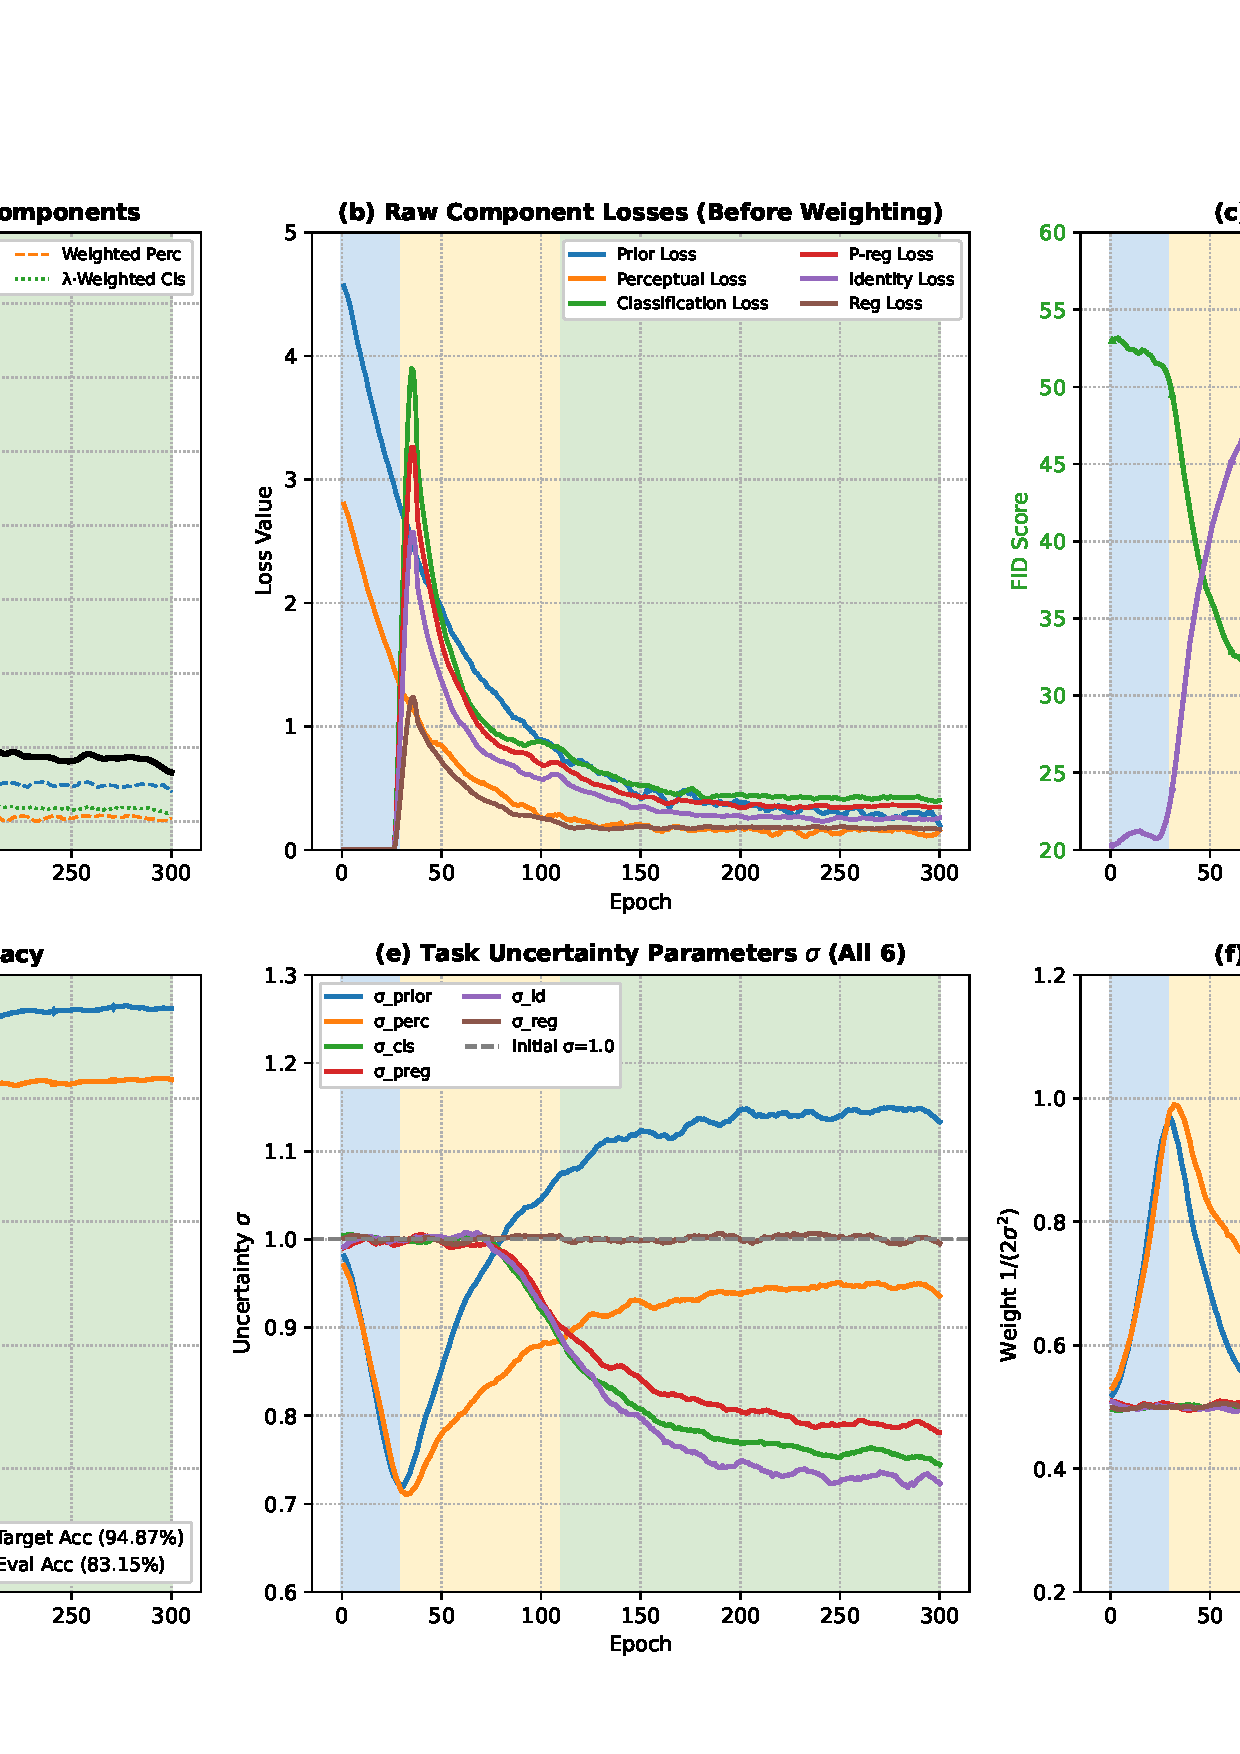
\includegraphics[width=\textwidth]{figures/mia_training_curves.pdf}
  \caption{MIA方法三阶段渐进式训练过程的损失与指标演化曲线}
  \label{fig:mia_training_curves}
\end{figure}
图~\ref{fig:mia_training_curves}展示三阶段训练的损失与指标演化。图中背景色区分训练阶段:阶段1(蓝色)为图像条件预热,阶段2(黄色)为混合条件过渡,阶段3(绿色)为纯标签条件适配。子图(a)展示总损失与部分核心损失的演化趋势,反映整体优化效果;子图(b)呈现全部损失项的独立演化,验证各损失函数的收敛性。子图(c)显示FID和KNN距离两项质量指标的变化,在阶段1图像条件预热阶段,由于仅建立图像到换脸的基础映射而未针对目标类别优化,FID维持在较高水平,KNN距离保持在极低值几乎无变化;阶段2引入标签条件后,随着混合系数$\lambda(t)$从0逐渐增长至1,标签条件的贡献逐步增强,两项指标开始显著改善,FID快速下降,KNN距离大幅跃升,充分体现了标签条件引导对目标类别特征匹配的关键作用;阶段3通过LoRA微调进一步优化,两项指标持续提升直至收敛,最终达到表~\ref{tab:mia_training_ablation}所示的三阶段训练结果。子图(d)展示目标准确率和评估准确率的提升过程,呈现与质量指标相似的演化规律。在阶段1,由于尚未建立标签到嵌入的映射,两项准确率保持在极低水平;阶段2引入标签条件后,准确率快速上升;阶段3进一步提升,最终收敛至表~\ref{tab:mia_training_ablation}的三阶段训练策略对应值。子图(e)展示任务不确定性参数$\sigma_i$的动态演化,扩散先验的$\sigma_{\text{prior}}$在阶段1保持较低水平确保生成质量,分类引导和身份一致性的$\sigma_{\text{cls}}$、$\sigma_{\text{id}}$在阶段2-3显著下降驱动攻击准确率提升;子图(f)展示对应的权重系数$1/(2\sigma_i^2)$的变化,清晰反映各任务重要性的自适应调整过程,该自动权重调整机制使框架无需人工超参数搜索即可在多目标间达到动态均衡。


\begin{table}[htbp]
  \centering
  \caption{模型反演方法损失项组合消融实验}
  \label{tab:mia_loss_ablation}
  \begin{tabular}{lcccc}
    \hline
    损失组合 & TarAcc & EvalAcc & FID & KNN Dist \\
    \hline
    仅扩散先验 $\mathcal{L}_{\text{prior}}$ & 7.85\% & 5.92\% & 53.47 & 0.4156 \\
    + 分类引导 $\mathcal{L}_{\text{cls}}$ & 77.24\% & 70.38\% & 36.82 & 0.5387 \\
    + 身份一致性 $\mathcal{L}_{\text{id}}$ & 92.56\% & 79.47\% & 29.15 & 0.6743 \\
    + 感知质量 $\mathcal{L}_{\text{perc}}$ & 94.87\% & 83.15\% & 23.26 & 0.7165 \\
    \hline
  \end{tabular}
\end{table}

表~\ref{tab:mia_loss_ablation}展示不同损失项组合对性能的影响。仅使用扩散先验损失时,缺乏针对目标分类器的优化信号,目标准确率仅为7.85\%。引入分类引导损失后,目标准确率显著提升至77.24\%。添加身份一致性损失,目标准确率达到92.56\%,评估准确率79.47\%。引入感知质量损失后,目标准确率达到94.87\%,评估准确率83.15\%,FID降至23.26。每增加一个损失项,评估准确率提升幅度均大于目标准确率,特别是身份一致性损失带来显著提升,表明这些损失项不仅提高攻击成功率,更增强生成样本的真实代表性和泛化能力,验证了多目标优化框架的必要性。


\subsection{可视化结果与分析}[Visualization Results and Analysis]
\label{sec:mia_visualization}

为直观展示模型反演方法的生成质量与多样性,图~\ref{fig:mia_grid_by_target}展示了针对不同目标类别的模型反演结果。其中每行对应一个源人脸,每列对应一个目标类别。该图验证了方法在固定源人脸条件下跨多个目标类别的攻击能力和生成多样性。从图中可观察到:同一行的生成图像继承了源人脸的姿态和表情属性,但在关键身份特征如面部轮廓、五官比例、发型等方面已转换为目标身份特征;同一列的生成图像虽源于不同源人脸,但在目标身份的视觉特征上保持高度一致,证明标签条件嵌入层成功学习目标类别身份表征。不同源人脸展现丰富的姿态变化、表情变化和光照条件,验证方法在不同源人脸条件下的鲁棒性。源人脸的姿态和表情属性被准确保留并迁移至目标身份,验证基于REFace的换脸先验能为模型反演任务提供强大结构引导,显著提升生成质量。

\begin{figure}[htbp]
  \centering
  \includegraphics[width=0.95\textwidth]{images/grid_by_target.jpg}
  \caption{模型反演方法针对不同目标类别的生成样本可视化。}
  \label{fig:mia_grid_by_target}
\end{figure}

生成图像不仅被目标分类器正确识别为对应类别,同时在视觉质量上呈现良好真实感,包括自然的肤色分布、清晰的五官轮廓以及合理的面部结构比例。利用REFace换脸先验显著提升生成质量,预训练的换脸模型为生成过程提供强大面部几何先验知识,使生成图像在面部结构一致性和光照自然度方面表现优异。标签条件嵌入层通过MLP网络成功实现从离散类别标签到连续身份表示空间的映射,不同类别的生成图像呈现明显身份区分度,验证标签条件嵌入机制的有效性。

上述可视化结果验证第四章提出的基于换脸先验迁移的多目标自适应模型反演方法在保持高攻击准确率的同时能显著提升重建图像的保真度和视觉质量,基于换脸先验的生成框架与标签条件嵌入机制的有机结合使方法在攻击有效性与生成真实感之间实现良好平衡,展现出在实际应用场景中的潜在威胁性。

\section{本章小结}
\label{sec:mia_summary}

本章提出基于换脸先验迁移的多目标自适应模型反演方法,利用预训练换脸模型的身份属性解耦机制,通过标签条件嵌入层建立离散类别标签与连续身份嵌入空间的映射,采用低秩适应(LoRA)微调技术以极少参数开销适配新的嵌入分布,设计渐进式三阶段训练策略实现从图像条件到标签条件的平滑模态迁移,结合多目标自适应优化框架动态平衡扩散先验、分类器攻击、身份一致性与感知质量等目标,并在推理阶段引入分类器引导采样机制提升攻击有效性,实现从类别标签到高保真攻击样本的生成。实验结果表明,该方法在多种目标分类器架构上均表现出优异的攻击准确率与生成保真度,消融实验验证了渐进式训练策略、LoRA微调与任务不确定性加权框架等核心模块的有效性。
% Local Variables:
% TeX-master: "../main"
% TeX-engine: xetex
% End:
